\begin{figure} 
\centering 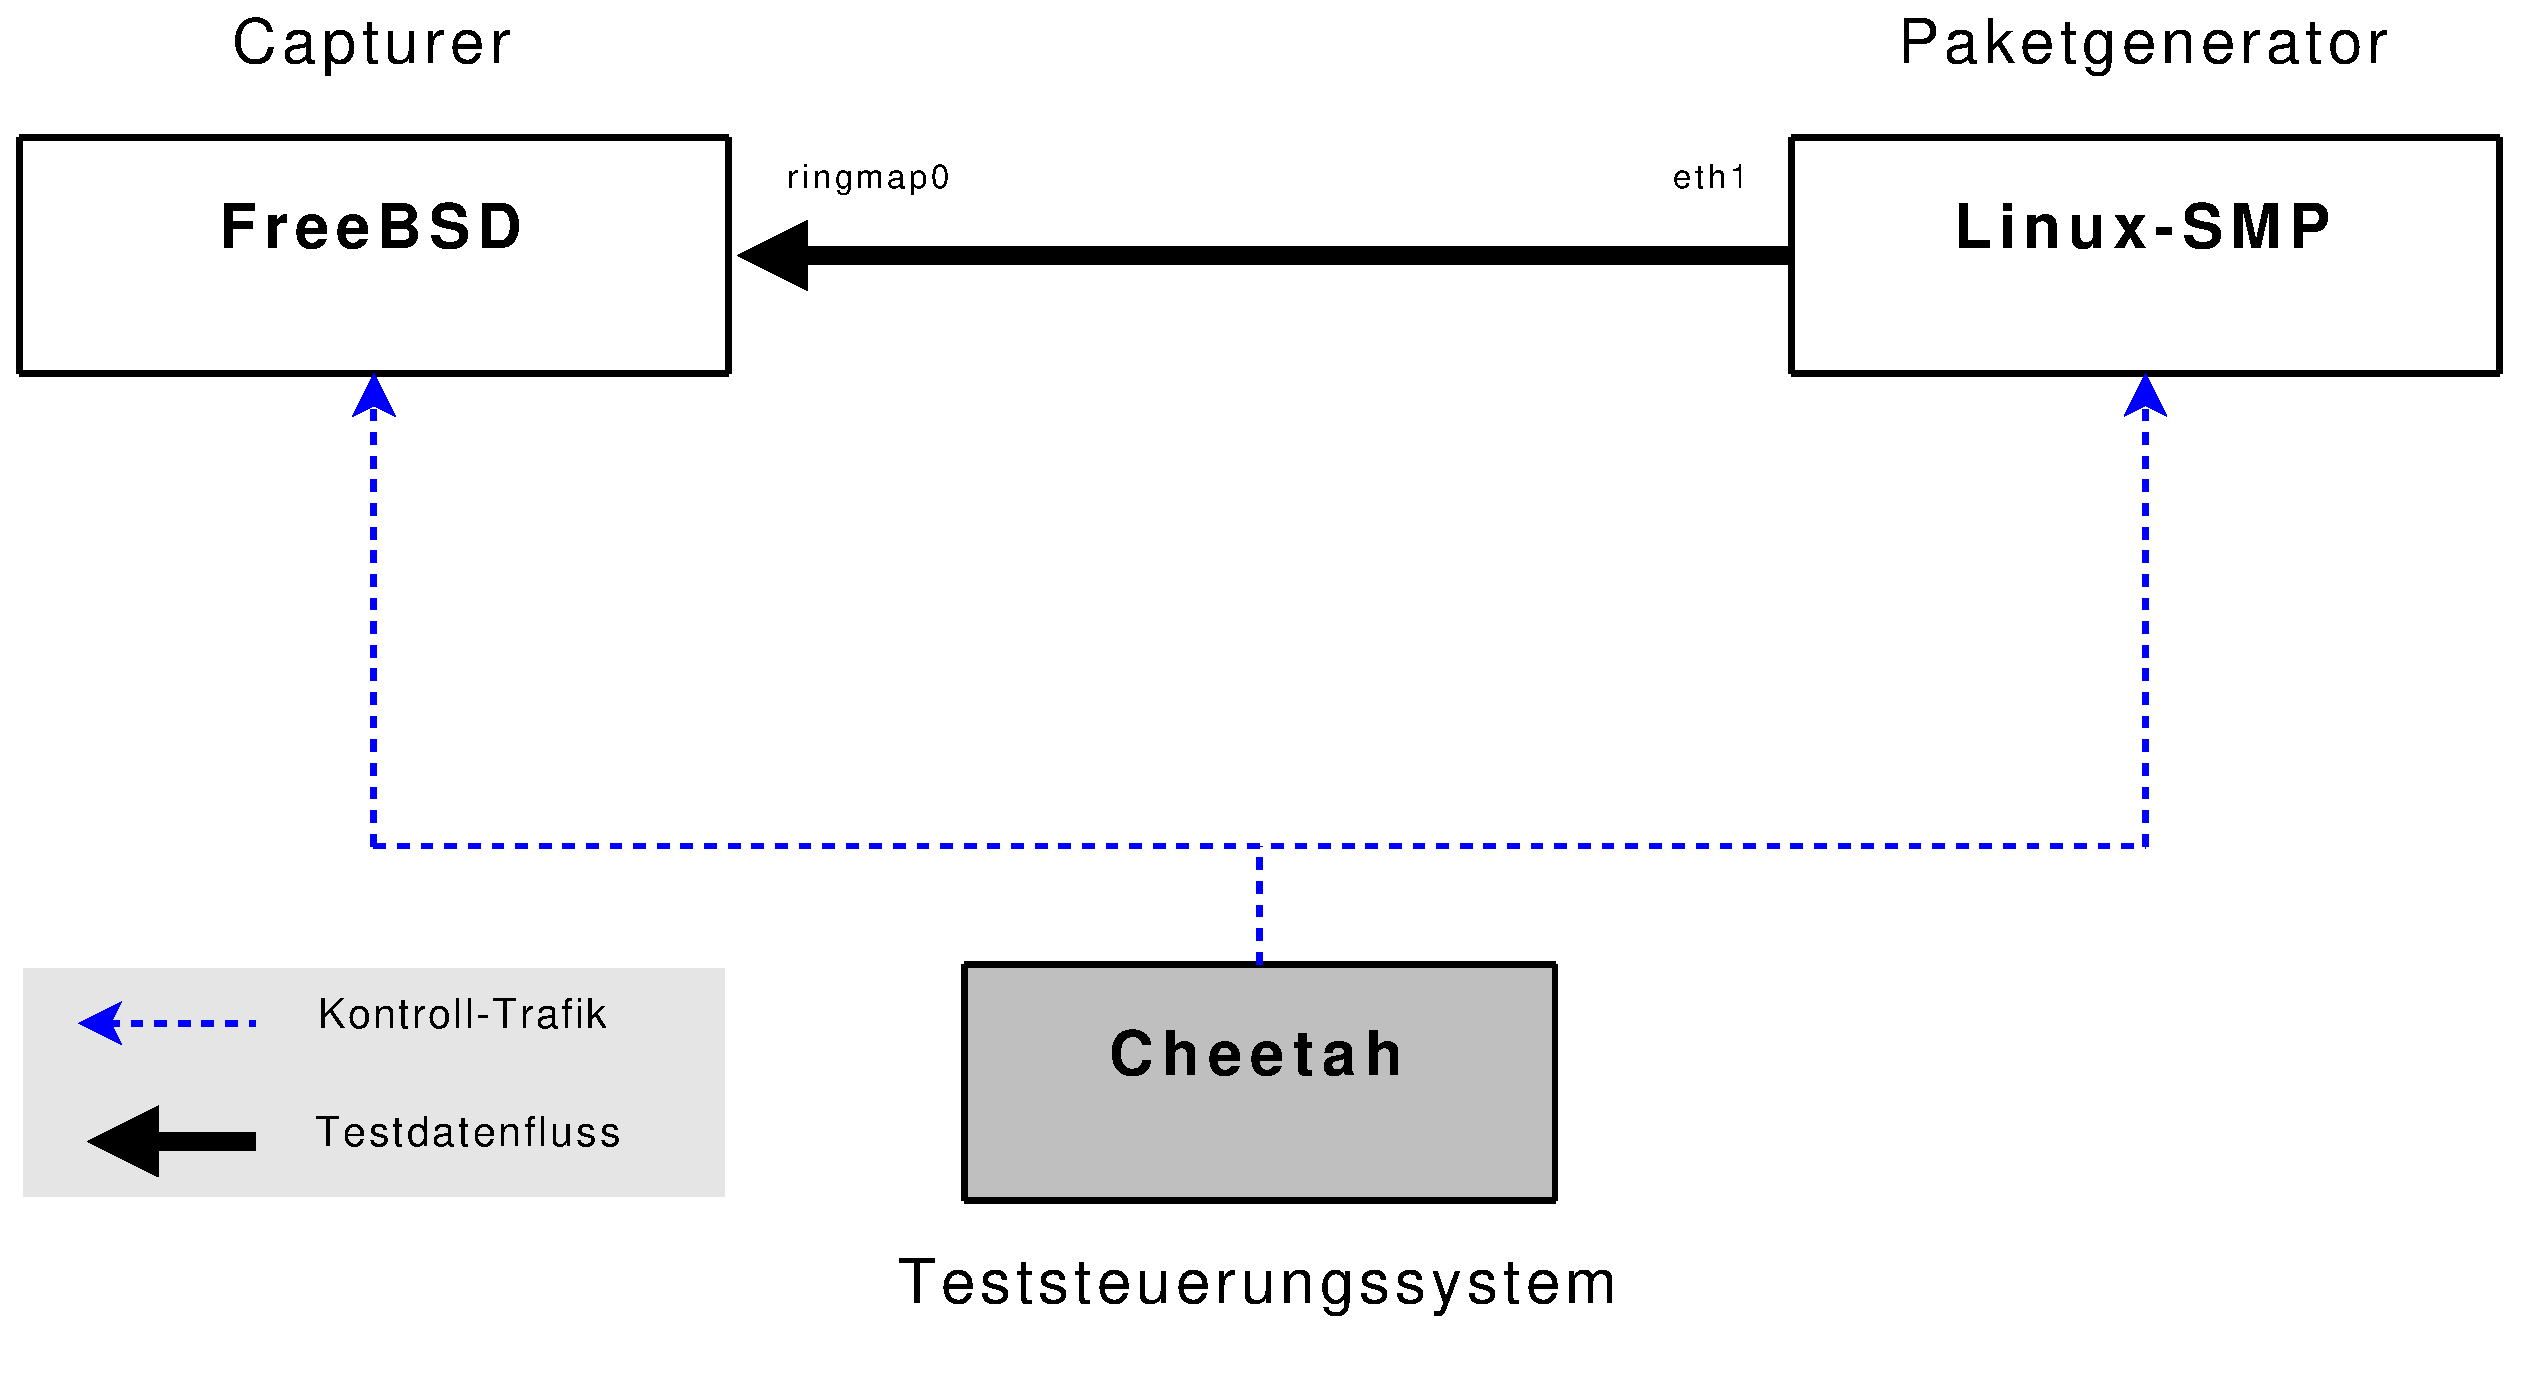
\includegraphics[width=5.5in]{bilder/Messaufbau}
\caption{Netzwerk-Diagramm des Testsbeds}
\label{img:test_aufbau}
\end{figure}
In diesem Kapitel werden die Ergebnisse des Leistungsvergleichs zwischen den
\emph{generischen} und den im Rahmen des Projektes entwickelten
\emph{ringmap}-Packet-Capturing-Stacks dargestellt. Für die Tests ist ein
Netzwerk mit drei Hosts aufgebaut. Das Netzwerkdiagramm der Testsumgebung ist
in Abbildung \ref{img:test_aufbau} dargestellt. Auf dem \textbf{Paketgenerator}
ist Verkehr mit unterschiedlichen Charakteristiken erzeugt und auf dem
\textbf{Capturer} erfasst. Dabei sind die Paketverluste und die
Systemlast während der Datenerfassung gemessen.
%
\ifthenelse{\boolean{BRIEF}}{}{   
Das \emph{ringmap}-Stack wird nicht nur mit unterschiedlichen Verkehrsmustern
untersucht. Für die Teststabläufe werden verschiedene Konfigurationsparameter
für das Betriebssystem und den Treiber eingesetzt, mit dem Ziel eine optimale
\emph{ringmap}-Konfiguration, die eine bestmögliche Leistung ermöglicht,
herauszufinden.\\\\
%
Die Performance des \emph{generischen} Stacks wurde bereits in mehreren
wissenschaftlichen Experimenten untersucht~\cite{fabian_da, pcin10gb_paper,
perfev_paper}. Aus diesem Grund werden mit dem \emph{generischen}-Stack nur
wenige Experimente durchgeführt, um die Performance von \emph{ringmap} und
\emph{generic} vergleichen zu können.
}

\subsection{Messaufbau}\label{sec:messaufbau}
Im Folgenden beschreibe ich die für Tests eingesetzten Knoten (Abbildung
\ref{img:test_aufbau}): 
\begin{itemize}
	\item Paketgenerator
		\begin{itemize}
			\item Ein leistungsfähigen Rechner zum Generieren des Test-Verkehrs.
			\item OS: Linux-SMP
			\item Linux Kernel Packet generator~\cite{linux_pktgen} wird für
				die Generierung des Netzverkehrs benutzt.
		\end{itemize}
	\item Capturer
		\begin{itemize}
			\item OS: FreeBSD mit \emph{generic} und \emph{ringmap}
				\begin{itemize}
					\item FreeBSD-7.2, i386-Kernel (32 Bit)
					\item Interrupt-Throttling default Parameter:
						\begin{itemize}
							\item 8000 Interrupts pro Sekunde maximal
						\end{itemize}
				\end{itemize}
			\item Hardware:
				\begin{enumerate}
					\item FreeBSD-1:
						\begin{itemize}
							\item \textbf{CPU:} AMD Athlon(tm) 64 Processor 2214.45-MHz
							\item \textbf{Netzwerkadapter:} PCI, Intel Dual Port Gigabit Ethernet Controller
						\end{itemize}
					\item FreeBSD-2:
						\begin{itemize}
							\item \textbf{CPU:} 4 x Intel(R) Xeon(R) CPU 1.60GHz
							\item \textbf{Netzwerkadapter:} PCIe, Intel HP NC360T PCIe DP Gigabit Server Adapter	 
						\end{itemize}
				\end{enumerate}
						\end{itemize}
	\item Teststeuerungssystem
		\begin{itemize}
			\item OS: Linux
			\item Scripte zur Teststeuerung.
		\end{itemize}
\end{itemize}
\ifthenelse{\boolean{BRIEF}}{}{  
\begin{figure} 
\centering 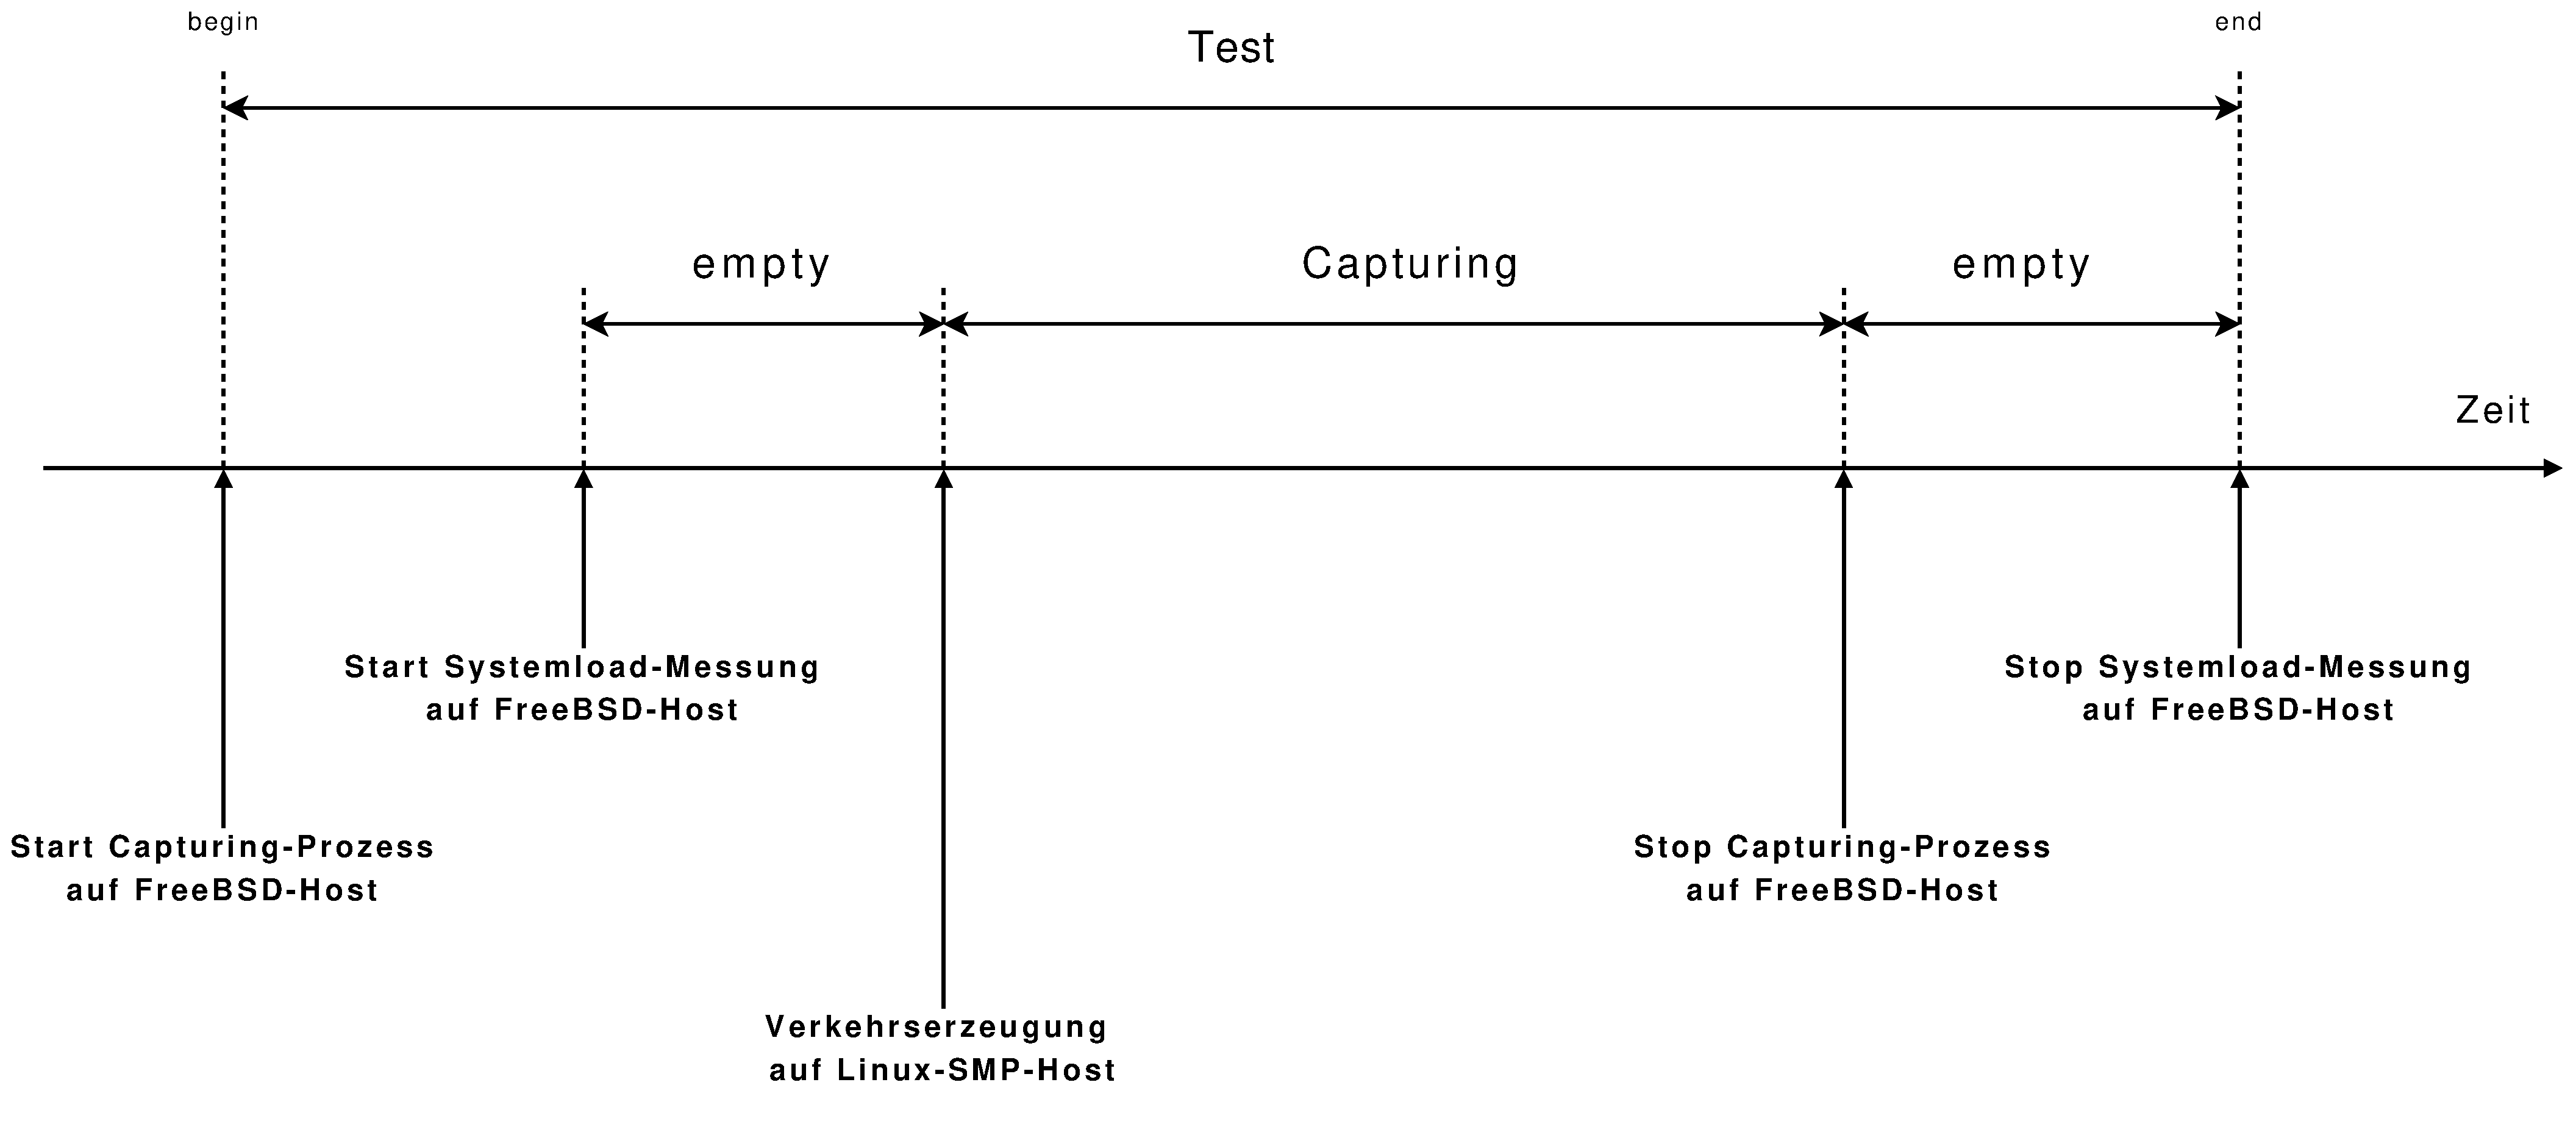
\includegraphics[width=6.5in]{bilder/Test_Zeit_Ablauf}
\caption{Testablauf}
\label{img:test_ablauf}
\end{figure}
\subsubsection{Testablaufspezifikationen}
Für die Testablauf-Steuerung wird ein Shellskript\footnote{SVN-URL:
\url{https://svn.net.t-labs.tu-berlin.de/svn/alexandre-da/src/70/scripts/dotests.sh}}
eingesetzt. Der Skript wird auf \emph{Cheetah} gestartet, und steuert durch
SSH-Verbindungen zu \emph{Capturer}- und \emph{Paketgenerator}-Host den Ablauf
jedes Testes.\\\\
Folgend beschreibe ich den Ablauf der Tests in Einzelschritten (siehe Abbildung
\ref{img:test_ablauf}): 
\begin{enumerate}
	\item SSH-Login auf \emph{FreeBSD}:
		\begin{enumerate}
			\item Starten Capturing-Prozess.
			\item Starten Systemload-Messung.
		\end{enumerate}
	\item SSH-Login auf \emph{Linux-SMP}:
		\begin{enumerate}
			\item Starten Verkehrserzeugung-Prozess
				\begin{itemize}
					\item Es wird Testdatenfluss generiert. Dabei wird eine
						bestimmte Anzahl von Paketen gleicher Länge erzeugt und
						zu dem \emph{Capturer} gesendet.
				\end{itemize}
			\item Speichern in einer Temp-Datei der Charakteristiken des
				erzeugten Verkehr: Bit-Rate, Paket-Rate.
		\end{enumerate}
	\item SSH-Login auf \emph{FreeBSD}:
		\begin{enumerate}
			\item Stop Capturing-Prozess
			\item Stop Systemload-Messung.
			\item Speichern in einer Temp-Datei der Systemload-Mess-Daten und
				Anzahl der empfangenen Pakete. 
		\end{enumerate}
	\item SSH-Login auf \emph{FreeBSD} und \emph{Linux-SMP}:
		\begin{itemize}
			\item Kopieren der gespeicherten Test-Daten von den \emph{FreeBSD} und
			\emph{Linux-SMP} auf \emph{Cheetah}
		\end{itemize}
\end{enumerate}
Jeder Test wird fünf mal wiederholt. Für die gemessenen Werte wird das
Arithmetisches Mittel und Standardabweichung berechnet, welche auf den Grafiken
in den folgenden Abschnitten dargestellt sind.

}
\subsubsection{Erzeugung von Verkehr}
Der Verkehr für die Tests wird mit
\emph{Linux-Kernel-Packet-Generator}(\emph{pktgen})~\cite{linux_pktgen} erzeugt.
\emph{pktgen} ist ein Linux-Kernel-Module, das benutzt wird um die UDP-Pakete
zu generieren und diese ins Netz zu senden. Für die Steuerung von \emph{pktgen}
wird das \verb+/proc+-Filesystem benutzt.\\\\
Der \emph{Linux-Kernel-Paket-Generator} wurde für die Experimente ausgewählt,
weil er mehrere Vorteile mit dem Unterschied zu den anderen Software (z.B.
Nemesis, Scapy, Iperf, etc\ldots) für die Erzeugung des Netz-Verkehr bietet. Vor
allem handelt es sich dabei um eine sehr hohe Paket-Rate, die mit \emph{pktgen}
erzeugt werden kann.
%
\ifthenelse{\boolean{BRIEF}}{}{  
Um eine hohe Paket-Rate bei Intel Ethernet Gigabit Adapter zu erzeugen, müssen
einige Eigenschaften des Netzwerkadapters beachtet werden, und zwar,
handelt es sich um \emph{Flow-Control}-Mechanismus.
}
%
\ifthenelse{\boolean{BRIEF}}{}{   
\subsubsection*{Flow-Control}
Unter dem Begriff \emph{Flow-Control} verstecken sich unterschiedliche 
Verfahren, die es erlauben, die Datenübertragung in einem Netz, die nicht synchron 
abläuft, so zu steuern, dass eine möglichst kontinuierliche Datenübermittlung ohne 
Paket-Verluste erfolgen kann. Das erfolgt sich dadurch, dass die Paketsendung 
im Fall eines schnelles Senders und eines langsamen Empfänger zeitweise unterbrochen 
wird.\\\\
%
Beim Intel Gigabit Netzwerkadapter ist der \emph{Flow-Control}-Mechanismus per Default
eingeschaltet, und das kann  bei der Verkehr-Generierung zu einigen  Problemen
führen. Erstens wird der \emph{Flow-Control}-Verkehr nicht von der
Capturing-Software wahrgenommen, benutzt aber Bandbreite, die wir für unsere
Test-Abläufe maximal benutzen wollen.  Zweitens, da unser Ziel im Erreichen
maximal hohe Paket-Rate liegt, ist in unserem Fall der \emph{Flow-Control} nur ein
Hindernis, der die Datentransferrate begrenzt. Deshalb muss es vor Beginn der
Experimente sowohl auf dem Capturing-Host, als auch auf dem
Paket-Generator-Host ausgeschaltet werden.
%
\subsubsection*{Ausschalten von Flow-Control auf dem Intel Gigabit Netzwerkadapter}
Unter Linux kann die Abschaltung von \emph{Flow-Control} beim Laden des
\emph{pktgen}-Modules an der Kommandozeile erfolgen: 
\begin{equation}
	\verb+# modprobe e1000 FlowControl=0+
\end{equation}
Unter FreeBSD wird \emph{Flow-Control} aus dem Treiber durch direkte Beschreibung 
des \emph{Receive-Control-Register} (\verb+RCTL+) ausgeschaltet (Listing \ref{code:flow_ctl_dis}):
\begin{lstlisting}[frame=single, caption={Funktion zur Ausschaltung des Flow-Control-Mechanismus. Die Funktion wird im ringmap-Treiber verwendet.}, captionpos={b}, label={code:flow_ctl_dis}]
void ringmap_disable_flowcontr(struct adapter *adapter)
{
	unsigned int ctrl; 
	ctrl = E1000_READ_REG(&(adapter)->hw, E1000_CTRL);
	ctrl &= (~(E1000_CTRL_TFCE | E1000_CTRL_RFCE));
	E1000_WRITE_REG(&(adapter)->hw, E1000_CTRL, ctrl);
}
\end{lstlisting}	
%
}
\subsubsection{Messung der CPU-Auslastung und der Paketverluste beim Capturing}
Auf dem FreeBSD-Host werden beim Test-Ablauf die auf dem Paketgenerator
generierten und gesendeten Pakete erfasst. Dabei wird die Anzahl der
empfangenen Pakete und die Systemload beim Capturing auf dem Capturer gemessen.
Bei allen Experimenten werden die erfasste Pakete nicht auf die Festplatte 
geschrieben, sondern nur im RAM gezählt.
%
\subsubsection*{Messung von Paketverlusten}
Für das Packet-Capturing wird eine einfache Anwendung implementiert, die für den
Paketzugriff die Bibliothek \emph{Libpcap} benutzt. In dieser Capturing-Anwendung ist
ein \emph{callback}-Funktion enthalten, die für jedes empfangene Paket
aufgerufen wird, und derer Aufgabe ist es, die empfangene Pakete zu zählen.
Das Paketverlust (\begin{math}P_{los}\end{math}) wird als Differenz zwischen 
den Anzahl der empfangenen (\begin{math}P_{rcv}\end{math}) und
der gesendeten Pakete (\begin{math}P_{send}\end{math}) berechnet:
	\begin{equation}
		P_{los} = P_{send} - P_{rcv}
		\label{equ:pktloss}
	\end{equation}
%
\subsubsection*{Messung von CPU-Auslastung}
Die CPU-Last wird auf FreeBSD über die \emph{sysctl}-Variable
\lstset{language=bash} \verb+kern.cp_time+ abgefragt:
\begin{lstlisting}[captionpos={b}, frame=single]
% sysctl kern.cp_time
kern.cp_times: 27281 1333 301046 513 1001093319
%
\end{lstlisting}
Bei der Abfrage der \verb+kern.cp_time+-Variable werden auf dem Standard-Output die Zeiten
ausgegeben, welche die CPUs seit dem Start des Betriebssystem jeweils im \verb+user+-,  
\verb+nice+-, \verb+syst+-, \verb+intr+- und \verb+idle+-Modus verbracht
haben.\\\\
Beim Präsentieren der Tests-Ergebnisse wird aber nicht die volle CPU-Last, die
aus den \verb+user+- \verb+nice+- \verb+syst+- \verb+intr+- \verb+idle+-Load
besteht, sondern lediglich die \textbf{Systemload} (\verb+syst+) angegeben.  Da
die Implementierung des neuen Stack hauptsächlich Kernel-Code betrifft,
interessiert uns vor allem die Systemload (\verb+syst+)\footnote{Aufgrund der
default Treiber-Einstellungen für Interrupt-Moderation, bleibt intr-Load
konstant. Deshalb interessiert uns Interrupt-Load auch nicht}.  Der Absicht der
Tests ist das Prüfen, ob unsere Entwurf-Ansätze korrekt sind, und ob sie zu dem
gewünschten Ziel führen. Anders gesagt, zu prüfen, ob die Ausführung des
Kernel-Codes vom neuen \emph{ringmap}-Capturing-Stack eine niedrigere
Systemlast als beim \emph{generic}-Capturing-Stack verursacht.
%
\ifthenelse{\boolean{BRIEF}}{}{   
Im System-Mode wird auch die Interrupt-Service-Routine(ISR) des Netzwerkadapters
ausgeführt (siehe Abschnitt \ref{sec:intr_behandlung}). Weil bei allen Tests
für die Interrupt-Rate-Steuerung \emph{Interrupt-Throttling} (siehe
Abschnitt \ref{sec:intr_coal}) verwendet wurde, blieb die Interrupt-Rate
während unserer Tests immer konstant, was auch immer eine konstante
Interrupt-Load (\verb+intr+: etwa $3\%$) verursacht hat. Aus diesem Grund 
können wir die Interrupt-Load in unseren Vergleichen ignorieren.
%liegt die Präsenz der Interrupt-Load auch außerhalb unserer Interessen.
%
\subsubsection*{Systemload-Messung}
Um die \textbf{Systemload} (\verb+syst+) während eines Test-Ablaufs zu messen, werden
die Werte des \verb+syst+-Counters vor Begin des Tests
(\begin{math}t_{begin}\end{math}) und nach dem Test (\begin{math}t_{end}\end{math}) 
gespeichert.  Durch die Differenz ergibt sich 
die Zeit, die CPUs während des Tests mit dem Ausführen des \verb+syst+-Codes zugebracht haben.  Diese Zeit entspricht aber nicht
exakt dem Testablauf, denn es sowohl zwischen den Messungsbeginn und Capturing
als auch zwischen Capturing-End und dem Mess-Ende (kurze)
Zeitintervalle (\begin{math}t_{empty}\end{math}) gibt, in
denen der \verb+syst+-Counter Zeit-Statistiken sammelt, die nicht während
Capturing entstehen, was das Endergebnis etwas verfälscht (siehe Abbildung \ref{img:test_ablauf}). \begin{math}t_{empty}\end{math} lässt sich messen, 
und zwar dadurch, dass man einen Test ohne Paketversand veranstaltet.\\\\
%
Aber dadurch, dass das Auftreten der Ereignisse, die das Ausführen des
Kernel-Codes verursachen (z.B. Interrupts oder Traps) unvorhersagbar ist, und,
dass die Anzahl von solchen Ereignissen pro Zeitintervall meistens variabel
bleibt, ist dieser Wert nicht exakt bestimmbar. Daher wurden vor Beginn aller Tests mehrere Messungen von 
\begin{math}t_{empty}\end{math} gemacht und ein durchschnittliches Wert 
\begin{math}\tilde{t}_{empty}\end{math}  berechnet.\\\\
%
Dann berechnet sich die Zeit (\begin{math}T_{syst}\end{math}), 
die sich CPUs während des Capturing im 
\verb+syst+-Mode verbracht haben durch: 
\begin{equation}
	T_{syst} = t_{end} - t_{begin} - \tilde{t}_{empty}
\end{equation}
Auf gleiche Weise lassen sich die CPU-Zeiten für \verb+user+- \verb+nice+- \verb+idle+- und \verb+intr+-Mode
berechnen. Dann berechnet sich die \textbf{Systemload} ($S$) als der prozentuelle Zeitanteil,
den die CPUs im \verb+syst+-Mode während des Tests verbracht haben 
durch:
\begin{equation}
	S = \frac{T_{syst} * 100}{(T_{user} + T_{nice} + T_{syst} + T_{intr} + T_{idle})}
\end{equation}

\subsection{Test-Parameter}\label{sec:test_params}
Für jeden Testablauf werden unterschiedliche Parameter eingesetzt, die sowohl
den Paket-Generierungs-Prozess als auch den Capturing-Prozess beeinflussen. Für
die Tests, die zum Vergleich des \emph{generic}- und \emph{ringmap}-Capturing-Stacks durchgeführt
wurden, werden lediglich die Paket-Generator-Parameter geändert, während die
Konfiguration der Treiber auf dem Capturing-Host konstant blieb.\\\\
Für die Auswertung der Performance des \emph{ringmap}-Stack wird eine größere 
Menge an Tests durchgeführt, um eine Konfiguration herauszufinden, bei der 
\emph{ringmap}-Stack mit optimaler Performance funktioniert.

\subsubsection{Parameter für die Generierung des Netz-Verkehrs}
Die Parameter, die für \emph{Linux Kernel Pakete Generator} gesetzt werden, 
erlauben es, die Paket-Größe und die Paket-Rate (dadurch auch Bit-Rate)
des generierten Verkehr zu steuern. Die Konfiguration von \emph{pktgen}
läuft über das \verb+/proc+-Filesystem ab.\\\\
In den Tests wurden folgende \emph{pktgen}-Parameter
eingesetzt\footnote{Eine detailierte Beschreibung der \emph{pktgen}-Parameter findet sich in
der Dokumentation~\cite{linux_pktgen}}:
\begin{description}
\item \verb+pkt_size+	
	\begin{itemize}
		\item Die Länge der erzeugten und gesendete Pakete. Beeinflusst auch 
			die Paket- und Bit-Rate des Verkehrs, denn je kleiner die Pakete sind ,
			desto größer wird der CPU-Aufwand für das Erzeugen einer bestimmten Datenmenge
			und desto höher die Anzahl der Bus-Transaktionen um diese Datenmenge 
			vom RAM zum Netzwerkadapter transferieren und ins Netz zu senden.
	\end{itemize}
\item  \verb+dstmac+	
	\begin{itemize}
		\item  Destination-MAC-Adresse. Wurde bei den Tests des
			\emph{generic}-Capturing-Stack absichtlich auf eine nicht dem NIC
			entsprechende MAC-Adresse gesetzt, damit die empfangenen Pakete
			nicht vom Protokoll-Stack bearbeitet werden, und dadurch keine
			zusätzliche Systemload beim Capturing erzeugen. 
	\end{itemize}
\item  \verb+delay+
	\begin{itemize}
		\item Zeitintervall in Nanosekunden zwischen den gesendeten Paketen.
			Beeinflusst die Paket- und damit auch die Bit-Rate des erzeugten
			Verkehr.
	\end{itemize}
\item  \verb+count+
	\begin{itemize}
		\item Anzahl der zu erzeugenden und zu sendenden Pakete. 	
	\end{itemize}
\end{description}

\subsubsection{Treiber-Parameter}
Die Parameter die für den \emph{ringmap}-Treiber gesetzt werden, beeinflussen
seine Performance, und können dadurch auf die Capturing-Performance einwirken.
Einige Parameter werden über \emph{sysctl}-Befehl~\cite{man_sysctl} gesetzt,
die anderen aber nur als Makrodefinitionen im Source-Code.
%
\begin{description}
	\item \verb+SLOTS_NUMBER+
		\begin{itemize}
			\item Ringpuffer-Größe: Anzahl der Ring-Slots bzw. der
				Paket-Puffer. Wird als Makrodefinition in der Datei
				\verb+fiveg_da.h+\footnote{\url{https://svn.net.t-labs.tu-berlin.de/svn/alexandre-da/src/70/em/fiveg_da.h}} gesetzt.
		\end{itemize}
	\item \verb+rx_processing_limit+
		\begin{itemize}
			\item Die maximale Anzahl der Pakete, die ein von der ISR geplanter
				Kernel-Thread bearbeiten darf. Wird über \emph{sysctl}-Befehl
				gesetzt. 
		\end{itemize}
\end{description}
}
\subsection{Ergebnisse}\label{sec:test_ergebnisse}
In diesem Kapitel werden die Ergebnisse der im Rahmen des Projektes
durchgeführten Experimente dargestellt. Der erste Abschnitt stellt die
Ergebnisse der Experimente mit dem neuen \emph{ringmap}-Packet-Capturing-Stacks dar. Es
werden die Systemload und Paketverluste beim Capturing in Abhängigkeit von der
Date-Rate des Verkehrs und der anderen Parameter dargestellt.\\\\
% 
Im Abschnitt \ref{sec:erg_verg} vergleichen wir die Performance des ringmap-
mit dem generic-Capturing-Stack, um den Performance-Gewinn durch den neuen
\emph{ringmap}-Capturing-Stack quantitativ zu bestimmen.

\subsubsection{Ringmap-Paket-Capturing-Stack}\label{sec:erg_ringmap_stack}
In diesem Abschnitt sind die Ergebnisse der Experimenten mit \emph{ringmap}-Capturing-Stack
dargestellt. Das Ziel der Experimenten die Capturing-Performance des \emph{ringmap}-Stacks 
in Abhängigkeit von den folgenden Parameter herauszufinden:
\begin{itemize}
\ifthenelse{\boolean{BRIEF}}{}{   
	\item Treiber-Konfigurationsparameter: \verb+rx_processing_limit+, \verb+SLOTS_NUMBER+.
}
	\item Paket-Ringpuffer-Größe
	\item Daten-Rate des erfassten Verkehr.
\end{itemize}

\subsubsection*{Paketverluste in Abhängigkeit von der Anzahl der Slots im  Paket-Ringpuffer}
\textbf{Das Ziel} dieses Experiments ist es, die Abhängigkeit der Paketverluste
während Capturing von der Größe des Paket-Ringpuffers (Ring-Buffer)
herauszufinden. In diesem Experiment ist eine Reihe von Tests durchgeführt. Für
alle Tests ist der Verkehr mit den kleinsten 64-Bytes Pakete und mit der maximal
erreichbaren Bit-Rate (c.a. $696Mbit/sec$) generiert.
%
\begin{itemize}
\item Konfiguration auf dem Capturer: 
\begin{itemize}
	\item \textbf{Hardware:} FreeBSD-2 (PCIe)
	\item \textbf{Betriebssystem:} FreeBSD \textbf{7.2}, \textbf{non-SMP Kernel}
\end{itemize}
\item Verkehrsparameter:
\begin{itemize}
	\item Paketlänge: 64-Bytes
	\item Paketmenge: 15000000
	\item Bit-Rate: etwa $696MB/sec$
\end{itemize}
\end{itemize}
\begin{figure} 
\centering 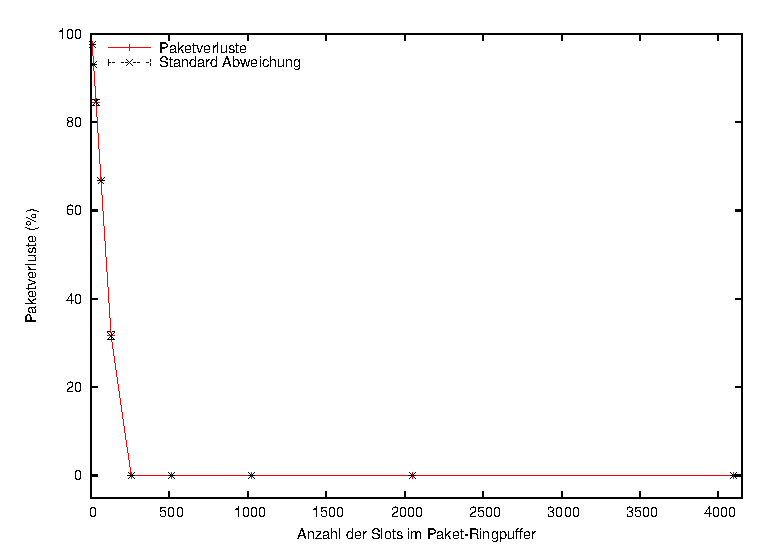
\includegraphics[width=5.5in]{plots/graphs/pktlos_single_bufsize.eps}
\caption{Paketverluste in Abhängigkeit von der Anzahl der Slots im Paket-Ringpuffer}
\label{img:plot_pktlos_puffs}
\end{figure}
%
\ifthenelse{\boolean{BRIEF}}{}{   
Beil allen durchgeführten Tests wird der Wert von \verb+rx_processing_limit+
auf $200$ gesetzt und der Wert \verb+SLOTS_NUMBER+ zwischen 8 und 4096
geändert. 
}
% 
\paragraph*{Paketverluste:}
In Abbildung \ref{img:plot_pktlos_puffs} sind die Paketverluste während
Capturing dargestellt.  Auf der X-Achse wird die Anzahl der Slots im
Ring-Buffer dargestellt.  Auf der Y-Achse die prozentuelle Anzahl der
Paketverluste. In allen durchgeführten Experimenten mit 256 oder mehr
Paket-Slots sind die Paketverluste relativ konstant und liegen unter $0.02\%$,
d.h. die Erhöhung der Anzahl der Slots ab 256 bringt keinen weiteren Gewinn
mehr. 
%
\ifthenelse{\boolean{BRIEF}}{}{   
\subsubsection*{Performance in Abhängigkeit von der maximalen Anzahl der pro Kernel-
Thread-Ablauf bearbeitende Paketen: rx\_processing\_limit}
\textbf{Das Ziel} dieses Experiments ist es, die optimale Werte für die
Variable \verb+rx_processing_limit+ zu finden, bei welchen die Paketverluste
und die Systemload minimal sind.\\\\
%
Konfiguration auf dem Capturer (\verb+FreeBSD+-Host): 
\begin{itemize}
	\item \textbf{Hardware:} FreeBSD-2	
	\item \textbf{Betriebssystem:} FreeBSD \textbf{7.2}, \textbf{single-CPU-Kernel}
	\item \textbf{Treiber:} 
		\begin{itemize}
			\item Paket-Ringpuffer-Größe: \verb+SLOTS_NUMBER+$=1024$
			\item Bit-Rate: etwa $696MB/sec$
		\end{itemize}
\end{itemize}
Verkehrsparameter:
\begin{itemize}
	\item Paketlänge: 64-Bytes
	\item Paketmenge: 15000000
\end{itemize} 
\begin{figure} 
\centering 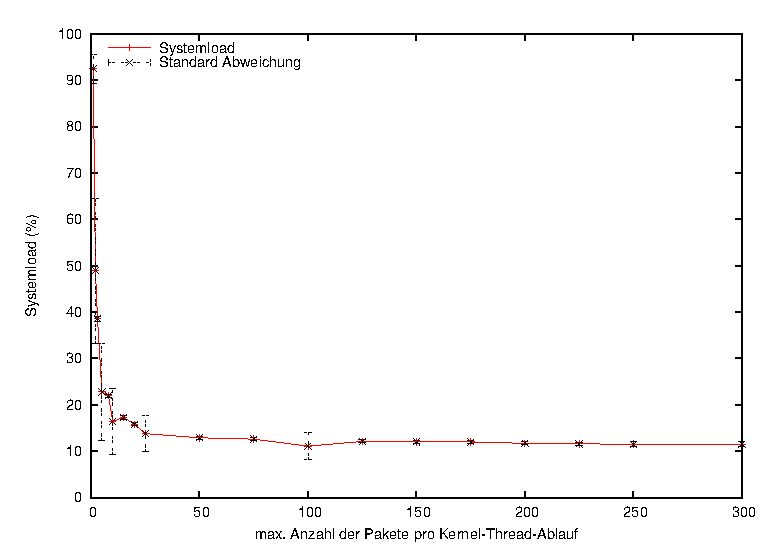
\includegraphics[width=5.5in]{plots/graphs/sysload_single_kts}
\caption{Systemload in Abhängigkeit von der maximalen Anzahl der pro Kernel-Thread-Ablauf
bearbeitende Pakete}
\label{img:plot_sysload_kts}
\end{figure} 
Bei Experimenten wird der wert von \verb+rx_processing_limit+ zwischen 1 und 300 
geändert.
\paragraph*{Paketverluste:} 
Bei allen durchgeführten Experimenten ergibt sich ein sehr kleiner Paketverlust
geringer als $0.02\%$ aller generierten Pakete.
\paragraph*{Soystemload:}
Die Ergebnisse des Systemload-Messungs-Experimentes sind in Abbildung
\ref{img:plot_sysload_kts} dargestellt.  Auf der X-Achse werden die Werte der
Variable \verb+rx_processing_limit+ dargestellt, auf der Y-Achse die Systemload
bei der Verkehrserfassung. Eine hohe Anzahl von Paketen pro Ablauf des
Kernel-Threads verursacht eine geringe Systemlast. Unsere Messungen zeigen dass
bei einer Einstellung $>50$ die Systemlast relativ Konstant unter $12\%$ bleibt. 
Die weitere Erhöhung des Wertes bringt keinen Gewinn mehr.
}
\subsubsection*{Performance in Abhängigkeit von Paketlänge, Bit-Rate und Paket-Rate}
\textbf{Das Ziel} des Experiments ist es, die Abhängigkeit der
Capturing-Performance von der Paketsgröße und Daten-Rate im Netzverkehr
herauszufinden.
%
\begin{itemize}
\item Konfiguration auf dem Capturer: 
\begin{itemize}
	\item \textbf{Hardware:} FreeBSD-2
	\item \textbf{Betriebssystem:} FreeBSD \textbf{7.2}, \textbf{non-SMP Kernel}
	\item \textbf{Treiber:} 
		\begin{itemize}
			\item Paket-Ringpuffer-Größe: 1024 Slots
		\end{itemize}
\end{itemize}
\item Verkehrsparameter:
\begin{itemize}
	\item Paketlängen: 64- , 200-, 300-Bytes
	\item Paketmengen: 15000000
\end{itemize}
\end{itemize}
%
\paragraph*{Paketverluste:} Bei allen Experimenten ergibt sich für Paketgrößen
über 200 Bytes die Paketerfassungsrate $100\%$. Nur in den Experimenten mit der
kleinsten Paketgröße von 64-Bytes und nur bei der höchsten erreichte Bit-Rate
von $627 MB/sec$ ergibt sich ein sehr kleines Paketverlust geringer als
$0.02\%$ aller generierten Pakete.
%
\paragraph*{Systemload:}
Die Ergebnisse der Systemload-Messung werden in den Abbildungen
\ref{img:plot_sysload_mbs} und \ref{img:plot_sysload_pps} dargestellt. Die
maximal erreichte Systemload beim Capturing in allen Experimenten liegt unter
$12\%$ und wird erreicht beim Capturing des Verkehrs mit den kleinsten
64-Bytes-Paketen.\\\\
%
In Abbildung \ref{img:plot_sysload_pps} wird die Systemload in Abhängigkeit von
der Paket-Rate dargestellt. Bei diesen Ergebnissen kann man deutlich sehen,
dass die Systemload beim Capturing von der Paket-Rate und nicht von der
Paket-Größe beeinflusst wird. Drei Verkehrsströme mit unterschiedlichen
Paketgrößen verursachen fast identisch gleiche Systemload (die Unterschiede
sind geringer als $0.5\%$) wenn die Paketraten in diesen drei Verkehrsströmen
gleich sind.  Dies lässt sich einfach erklären. Im neuen \emph{ringmap}-Treiber
wurden alle Paket-Kopie-Operationen und Speicherallozierungen entfernt. Der
Userspace-Prozess bekommt den Zugriff auf die Pakete sofort nach dem
DMA-Transfer. Aus diesen Gründen wird beim Capturing mit dem
\emph{ringmap}-Treiber im Kernelspace die geringstmögliche Arbeit erledigt, die
pro Paket-Puffer skaliert und nicht von der Paket-Größe abhängt.
%
\begin{figure} 
\centering 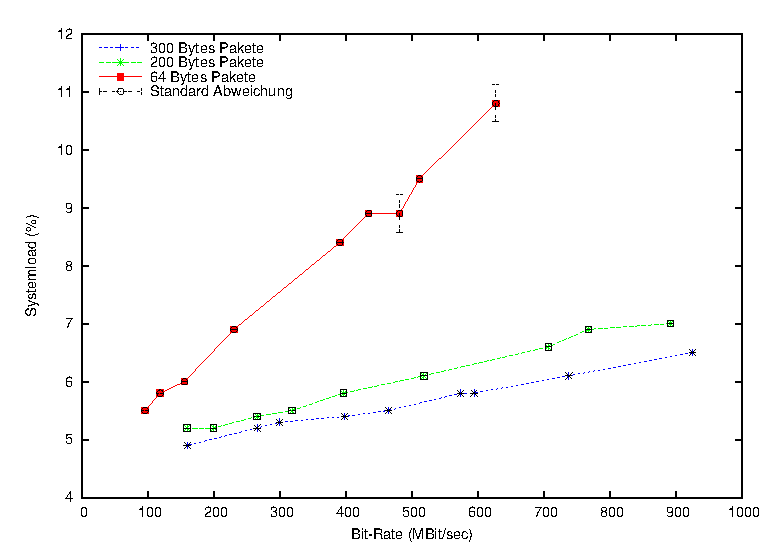
\includegraphics[width=5.5in]{plots/graphs/sysload_single_CPU_pcie_mbs}
\caption{Systemload in Abhängigkeit von Bit-Rate beim Capturing}
\label{img:plot_sysload_mbs}
\end{figure}
\begin{figure} 
\centering 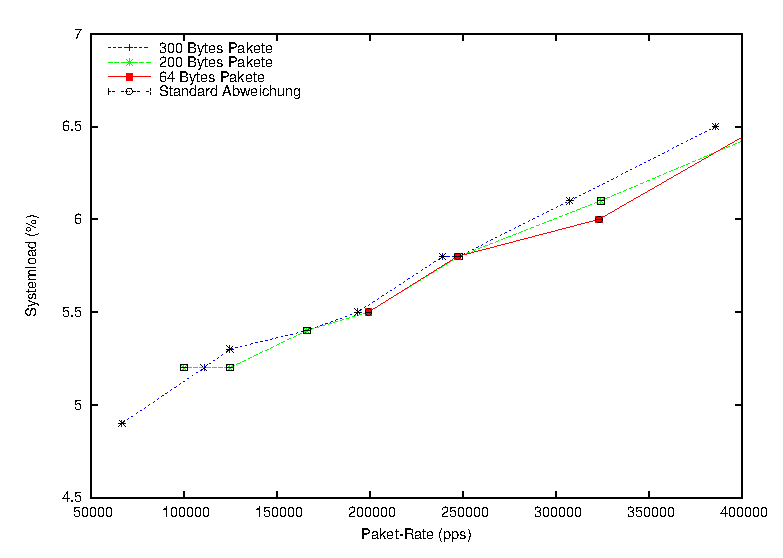
\includegraphics[width=5.5in]{plots/graphs/sysload_single_CPU_pcie_pps}
\caption{Systemload in Abhängigkeit von Paket-Rate beim Capturing}
\label{img:plot_sysload_pps}
\end{figure}
%
\ifthenelse{\boolean{BRIEF}}{}{   
\subsubsection*{Performance in Abhängigkeit von der Anzahl der CPU's}
\textbf{Das Ziel} des Experiments ist es, die Paketverluste beim Capturing 
in Abhängigkeit von der Anzahl der CPUs auf dem Capturing-System zu messen.\\\\
%
Konfiguration auf dem Capturer (\verb+FreeBSD+-Host): 
\begin{itemize}
	\item \textbf{Hardware:} FreeBSD-2	
	\item \textbf{Betriebssystem:} FreeBSD \textbf{7.2}, \textbf{single-CPU-Kernel}, \textbf{SMP}-Kernel
	\item \textbf{Treiber:} 
		\begin{itemize}
			\item Paket-Ringpuffer-Größe: 1024 Slots
		\end{itemize}
\end{itemize}
Verkehrsparameter:
\begin{itemize}
	\item Paketlänge: 64-Bytes
	\item Paketmenge: 15000000
\end{itemize}
%
Bei diesem Experiment werden für das Capturing unterschiedliche FreeBSD-Kerne
eingesetzt.  Bei einem Experiment läuft das Capturing mit dem SMP-Kernel, bei
dem anderen wird ein Kernel ohne SMP-Funktionalität verwendet. Für beide Tests
wird der Verkehr aus 64-Byte-Paketen generiert und gesendet. Die Ergebnisse des
Experiments sind in Abbildung \ref{img:plot_pktlos_single_vs_smp_mbs} zu sehen.
Auf der X-Achse ist die generierte Datenrate dargestellt. Auf der Y-Achse die
absolute Zahl der Paketverluste. Die durchschnittliche Anzahl der Paketverluste
für die Experimente mit einem SMP-Kernrel wird mit blauen Plus-Zeichen, die mit
dem Single-Kernel mit grünen Quadraten dargestellt. Die Paketverluste sind in
beiden Fällen im Verhältnis zur generierten Paketrate gering, steigen im Fall
des SMP-Kernels aber ab 400MBit/s stark an, bis auf 800 verlorene Pakete pro
Experiment.\\\\ 
%
Der SMP-Kernel Zeigt etwas schlechteres Performance. Der Grund dafür kann ein
Datenlokalitäts-Problem sein. Die unterschiedliche CPU-Kerne haben mindestens
einen eigenen Daten-Cache-Level, was Cache-Misses bei der Datenbearbeitung
verursachen kann. Dies war wahrscheinlich der Grund für die höheren
Paketverluste auf dem SMP-System.  Dennoch ist die Systemload beim Capturing
mit einem Single-CPU-Kernel geringer als $12\%$. Das heißt, dass eine CPU
problemlos das Capturing des Verkehrs bis 1Gbit schafft.
\begin{figure} 
\centering 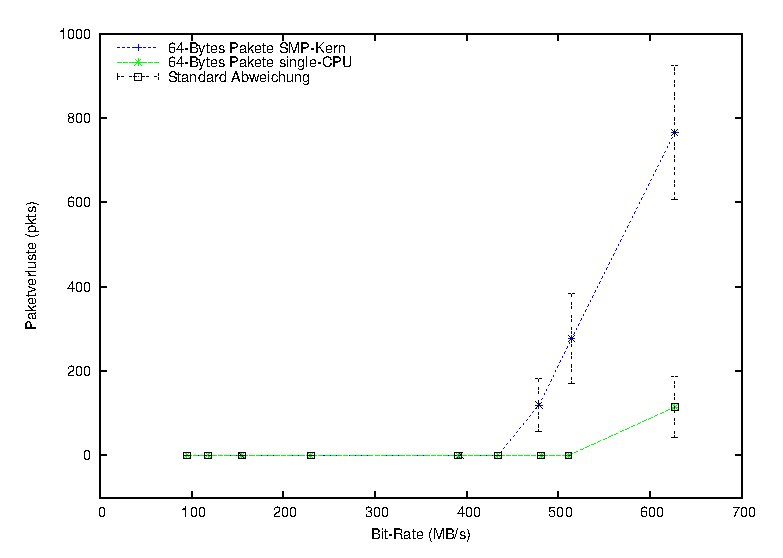
\includegraphics[width=5.5in]{plots/graphs/pktloss_single_vs_SMP_PCIe_mbs}
\caption{Paketverluste in Abhängigkeit von Paket-Rate beim Capturing auf einem SMP und single-CPU-System}
\label{img:plot_pktlos_single_vs_smp_mbs}
\end{figure}

\subsubsection*{Performance in Abhängigkeit von der PCI-Bus-Variante}
\textbf{Das Ziel} des Experimentes ist es die Capturing-Performance des
\emph{ringmap}-Stacks beim konventionellen PCI zu messen.\\\\
%
Konfiguration auf dem Capturer (\verb+FreeBSD+-Host): 
\begin{itemize}
	\item \textbf{Hardware:} FreeBSD-1
	\item \textbf{Betriebssystem:} FreeBSD \textbf{7.2}, \textbf{single-CPU-Kernel}
	\item \textbf{Treiber:} 
		\begin{itemize}
			\item Paket-Ringpuffer-Größe: 1024 Slots
		\end{itemize}
\end{itemize}
Verkehrsparameter:
\begin{itemize}
	\item Paketlänge: 64-Bytes
	\item Paketmengen: 15000000
\end{itemize}
\paragraph*{Paketverluste:}
Die Ergebnisse des Tests sind in Abbildung \ref{img:plot_pktlos_pci_mbs} zu
sehen. Auf der X-Achse wird die generierte Datenrate dargestellt. Auf der
Y-Achse der prozentuelle Anteil der Paketverluste. Der Rechnersystem mit dem
konventionellen \textbf{PCI} zeigt wesentlich schlechtere Paketerfassungsrate
beim Capturing als \textbf{PCIe}. Die Paketverluste entstehen sogar bei den
Verkehr mit großen Paketen (700- und 1500-Bytes) wenn die Bit-Rate über $800
MB/sec$ liegt. Verkehr, der ausschließlich die kleinsten 64-Bytes-Pakete
enthält, wird zu auf etwa $50\%$ erfasst. Das ist auch verständlich. Denn mit
den kleinsten Paketen wird auch die höchste Paket-Rate erzeugt ($>1000000
pkts/sec$).  Und dadurch, dass PCI-Bussystem einen großen Overhead beim
Transfer von Daten in den RAM hat (siehe Abschnitt \ref{sec:grund_bussyst})
schafft es es nicht, den Datentransfer bei einer so hohen Daten-Rate in den RAM
zu bewältigen.

\paragraph*{Systemload:}
Die Ergebnisse des Tests sind in Abbildung \ref{img:plot_sysload_pci_mbs}
präsentiert.  Die maximal erreichte Systemload liegt unter $13\%$, und damit in
der selben Größenordnung beim Verkehrerfassung auf dem Rechnersystem mit dem
\textbf{PCIe}-Bus. Da die Systemload so klein ist, ist sichergestellt, dass die
deutlichen Paketverluste beim 64-Bytes-Paket-Verkehr, nicht wegen der
Ineffizienz der Software oder zu niedrigeren Prozessor-Bus-Bandbreite
(Kopie-Operationen) entstehen.  Die Ursache der Paketverlusten liegt bestimmt
auf der Hardwareseite und bei diesen Experimenten ist der PCI-Bus-System sehr
wahrscheinlich der Grund dafür.
\begin{figure} 
\centering 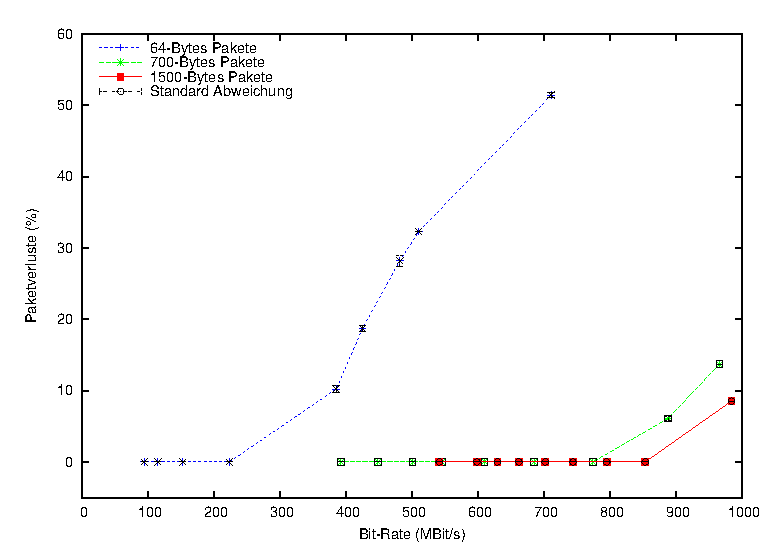
\includegraphics[width=5.5in]{plots/graphs/pktloss_PCI_mbs.eps}
\caption{Paketverluste in Abhängigkeit von der Bit-Rate beim Capturing auf dem Rechner mit dem konventioneller PCI-Bus}
\label{img:plot_pktlos_pci_mbs}
\end{figure}

\begin{figure} 
\centering 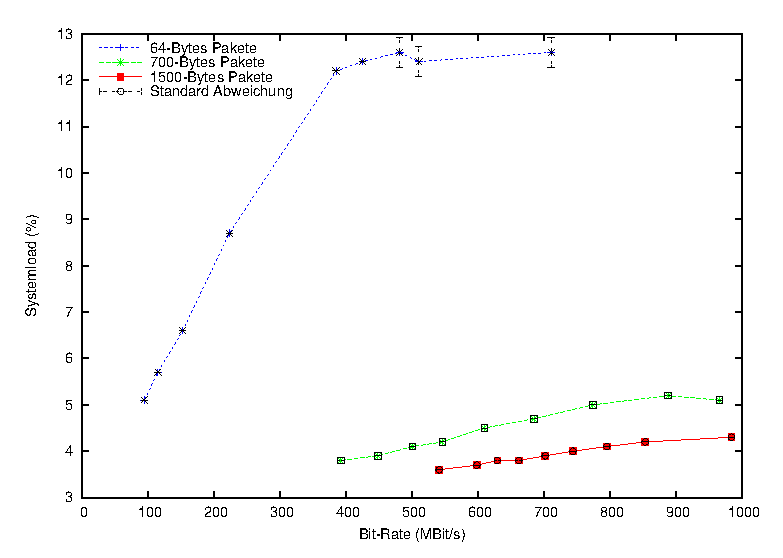
\includegraphics[width=5.5in]{plots/graphs/sysload_PCI_mbs.eps}
\caption{Systemload in Abhängigkeit von Bit-Rate beim Capturing. Konventioneller PCI-Bus}
\label{img:plot_sysload_pci_mbs}
\end{figure}
}
\subsubsection{Vergleich generic- mit ringmap-Paket-Capturing-Stack}\label{sec:erg_verg}
\textbf{Das Ziel} dieses Experiments ist es, die Capturing-Performance von 
\emph{ringmap}-Capturing-Stack mit dem \emph{generic}-Capturing-Stack
zu vergleichen.\\\\
%
Konfiguration auf dem Capturer: 
\begin{itemize}
	\item \textbf{Hardware:} FreeBSD-2 
	\item \textbf{Betriebssystem:} FreeBSD \textbf{7.2}, \textbf{non-SMP Kernel}
	\item \textbf{Treiber:} 
		\begin{itemize}
			\item Paket-Ringpuffer-Größe: 1024 Slots
			\item BPF-Puffer-Größe: 10MB
		\end{itemize}
\end{itemize}
Verkehrsparameter:
\begin{itemize}
	\item Paketlängen: 64-, 200-, 300-Bytes
	\item Paketmengen: 5000000-, 10000000-, 15000000 Pakete 
\end{itemize}

\paragraph*{Paketverluste:}
In Abbildung \ref{img:plot_pktlos_ringmap_vs_generic_mbs} sind die
Paketverluste dargestellt.  Auf der X-Achse wird die generierte Datenrate
dargestellt. Auf der Y-Achse der prozentuelle Anzahl der Paketverluste.  Bei
allen Tests entstanden die Paketverlust bei \emph{generic}-Stack lediglich für
Pakete der Größen 200 und 64 Bytes.  Dabei kann der \emph{generic}-Stack für
die 64-Bytes-Pakete bei der Bit-Rate von 393Mbit/s und höher
(entsprechende Paket-Rate $> 819545$) nur eine konstante Anzahl von Paketen
erfassen, etwa 262147 Pakete, unabhängig von der generierte Paketmenge. 

\paragraph*{Systemload:}
Die Ergebnisse der Systemload-Messung sind in Abbildung
\ref{img:plot_sysload_ringmap_vs_generic} dargestellt. Auf X-Achse wird die
generierte Datenrate dargestellt. Auf der Y-Achse die Systemload.  Bei
Erfassung der Verkehr mit dem \emph{generic}-Stack liegt die Systemload
wesentlich höher als beim \emph{ringmap}-Stack. Dies erklärt sich dadurch, dass
der \emph{generic}-Stack für jedes Paket mehrere Kopie-Operationen im
Kernelspace ausführt und für den Paketzugriff von der Userspace einen
Systemaufruf verwendet. Bei hohen Daten-Raten ist diese Vorgehensweise des
\emph{generic}-Stack nicht mehr effizient.
\begin{figure} 
\centering 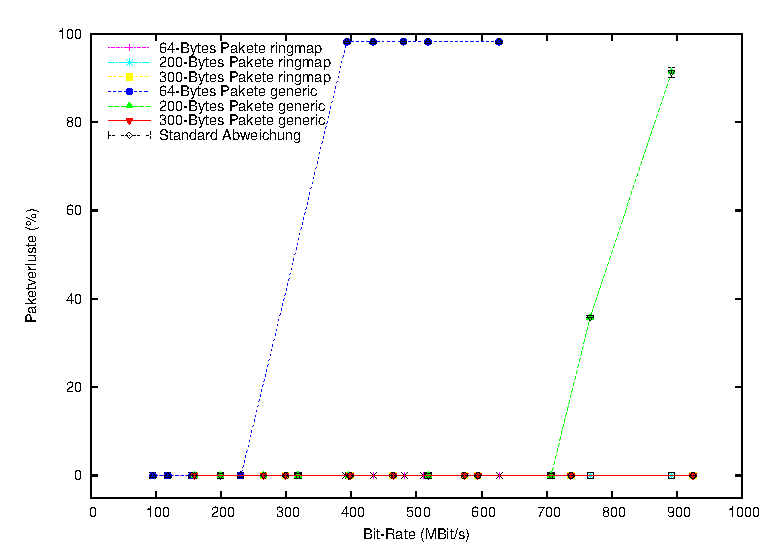
\includegraphics[width=5.5in]{plots/graphs/pktloss_generic_vs_ringmap_mbs.eps}
\caption{Paketverluste in Abhängigkeit von Bit-Rate beim Capturing. Vergleich ringmap- und generic-Packet-Capturing-Stacks}
\label{img:plot_pktlos_ringmap_vs_generic_mbs}
\end{figure}
\begin{figure} 
\centering 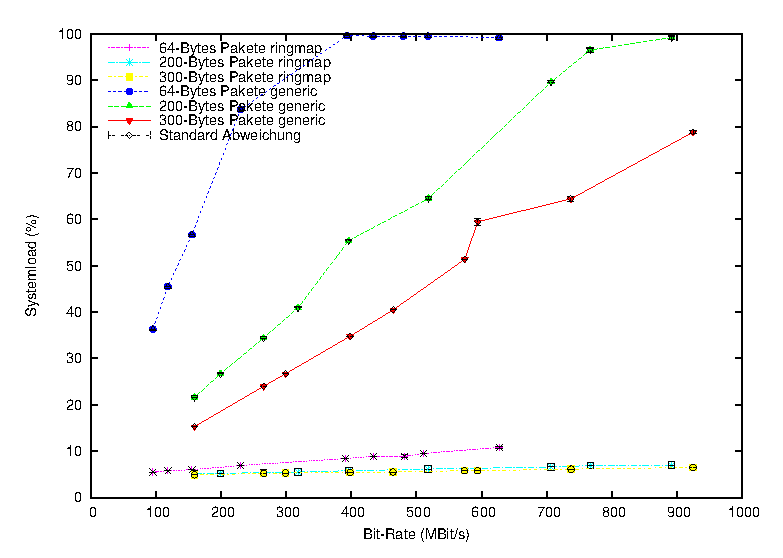
\includegraphics[width=5.5in]{plots/graphs/sysload_generic_vs_ringmap_mbs.eps}
\caption{Systemload in Abhängigkeit von Bit-Rate beim Capturing. Vergleich ringmap- und generic-Packet-Capturing-Stacks}
\label{img:plot_sysload_ringmap_vs_generic}
\end{figure}
